\documentclass[prb,preprint]{revtex4-1} 
\raggedbottom
\usepackage{amsmath}
\usepackage{amsfonts}
\usepackage{graphicx}

\begin{document}

\section{Results and Analysis}

Here we have two sets of data which are shown in Fig \ref{CvsV} and Fig \ref{Lin_Fit}. In Fig \ref{CvsV} the distribution of energies which are transferred to electrons within the cathode material by photons from the source are demonstrated to have a statistical nature. Since electrons are fermions, the exact distribution is described by the Fermi-Dirac distribution,
\begin{equation}
N(E,T)=\frac{1}{e^{(e_i-\mu)/(k_bT)}+1}
\end{equation}
where $e_i$ is the energy of a given particle state, $\mu$ is the Fermi energy plus the chemical potential at that state, $k_b$ is Boltzmann's constant, $T$ is the temperature, and $N(E,T)$ describes the probability of finding a particle at a given $E$ or $T$. By increasing the retarding voltage between the cathode and anode, the number of electrons reaching the anode are reduced until only the electrons which are at the Fermi level, $\mu$, are capable of overcoming the potential difference. As such we should expect that Fig \ref{CvsV} would closely resemble the distribution which can be predicted by the Fermi-Dirac distribution. In addition to the raw data an arbitrary function of the form of $N(E,T)$ has been overlaid to demonstrate that our measurements are indeed a reflection of the Fermi-Dirac distribution.

 
\begin{figure}[h!]
\centering
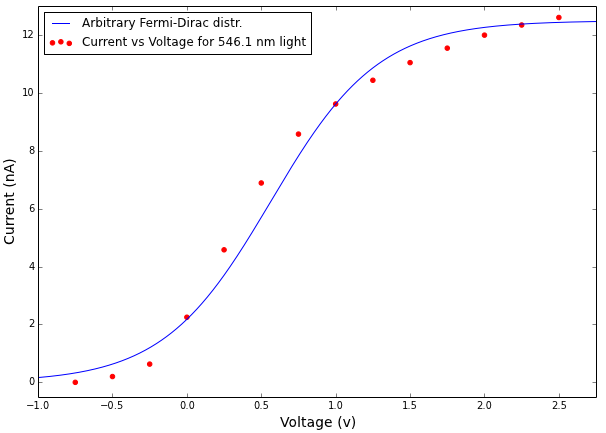
\includegraphics[width=.75\textwidth]{CvsV_overlay.png}
\caption{The measurements of current versus voltage}
\label{CvsV}
\end{figure}

\newpage

In Fig \ref{Lin_Fit} we make a linear fit function of the form $y=mx+b$ where $y$ is the stopping voltage, $m$ is analogous to $h/e$, $x$ is the light source frequency, and $b$ can be said to be $\phi$ or $W/e$. By optimizing this function using a least squares approximation of the value $m$ and $b$ we can determine the experimental values for both Plank's constant and the work function of the cathode material.

\begin{figure}[h!]
\centering
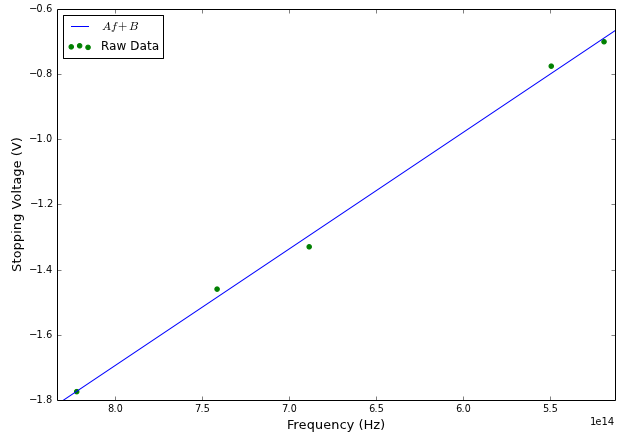
\includegraphics[width=.71\textwidth]{Lin_Fit.png}
\caption{The dependance of stopping voltage versus light source frequency}
\label{Lin_Fit}
\end{figure}

In order to ensure that the measured values are truly accurate, a test of the relationship between intensity and stopping voltage was conducted. During the test it was found that for 546.1 nm light the stopping voltage remained constant at a value of 0.79 V in spite of a changing source apertures. As expected the only observed effect which resulted from the intensity of light was an increases in the observed current with no changes to the energy distribution of the electrons. With confidence that the intensity of light had no effect on stopping voltage we find that the experimental value of $h$ is $5.7\pm0.2\times10^{-34}$ Js which is in disagreement with the accepted value of $6.626\time10^{-34}$ Js\cite{const} while the experimental value for $W$ was found to be $1.9\times10^{-19}\pm5\times10^{-28}$ J. Based upon these values for $h$ and $W$ we determine the threshold frequency of the cathode material to be $3.3\pm0.1\time10^{14}$ Hz.
\newpage

\begin{thebibliography}{99}

\bibitem{const} P.J. Mohr, B.N. Taylor, and D.B. Newell (2011), "The 2010 CODATA Recommended Values of the Fundamental Physical Constants" (Web Version 6.0).

\end{thebibliography}

\end{document}
